\documentclass{ximera}

\input{../preamble.tex}

\outcome{Define a cross product.}
\outcome{Compute cross products.}
\outcome{Use cross products in applied settings.}

\title[Dig-In:]{The cross product}

\begin{document}
\begin{abstract}
  The cross product is a special way to multiply two vectors in
  three-dimensional space.
\end{abstract}
\maketitle

There is no ``nice'' way to ``multiply'' two vectors and obtain
another vector in general. However, in the special case of $\R^3$,
there is an important multiplication operation called ``the cross
product.''

The cross product is linked inextricably to the determinant, so we
will first introduce the determinant before introducing this new
operation. See \href{http://www-groups.dcs.st-and.ac.uk/history/HistTopics/Matrices_and_determinants.html}{this paper}
for a discussion of the history of the idea of a \textit{determinant}.


\section{Determinants}

\begin{definition}
  Given a $2\times2$ matrix, the \dfn{determinant} is given by:
  \[
  \det
  \begin{bmatrix}
    a & b\\
    c & d
  \end{bmatrix}
  =
  \begin{vmatrix}
    a & b\\
    c & d
  \end{vmatrix}
  = ad -bc.
  \]
\end{definition}
Why would anyone ever be interested in this? Well to start, given nonzero vectors
\[
\vec{v} = \vector{a,b}\quad\text{and}\quad\vec{w}=\vector{c,d}
\]
we can form a parallelogram:
\begin{image}
\begin{tikzpicture}
  \draw[fill=fill1!50!white,draw=none]
  (0, 0)         % starting point
  -- ++(5,1)     % move along this vector
  -- ++(2,3)     % then along this vector
  -- ++(-5,-1)   % then back along that vector
  -- cycle;      % and back to where you started
  \draw[->,ultra thick,penColor] (0,0) -- (5,1);
  \draw[->,ultra thick,penColor2] (0,0) -- (2,3);
  \draw[->,ultra thick,dashed,penColor2] (5,1) -- (7,4);
  \draw[->,ultra thick,dashed,penColor] (2,3) -- (7,4);
  \node[above,penColor] at (2.5,.5) {$\vec{v}$}; %% <a,b>
  \node[below right,penColor2] at (1,1.5) {$\vec{w}$}; %% <c,d>
\end{tikzpicture}
\end{image}
The determinant gives the (signed) area of this parallelogram, where
the sign of the area is given by the sign of the angle between
$\vec{v}$ and $\vec{w}$. To understand why this is true, make a
rectangle around the parallelogram:
\begin{image}
\begin{tikzpicture}
  \draw[fill=fill1!50!white,draw=none]
  (0, 0)         % starting point
  -- ++(5,1)     % move along this vector
  -- ++(2,3)     % then along this vector
  -- ++(-5,-1)   % then back along that vector
  -- cycle;      % and back to where you started

  \draw[fill=fill5,draw=none] (5, 0) -- (7,0) -- (7,1) -- (5,1) -- cycle;
  \draw[fill=fill5,draw=none] (0, 3) -- (2,3) -- (2,4) -- (0,4) -- cycle;

  \draw[fill=fill3,draw=none] (0, 0) -- (5,0) -- (5,1) -- cycle;
  \draw[fill=fill3,draw=none] (2,3) -- (7,4) -- (2,4) -- cycle;

  \draw[fill=fill4,draw=none] (0, 0) -- (2,3) -- (0,3) -- cycle;
  \draw[fill=fill4,draw=none] (5, 1) -- (7,1) -- (7,4) -- cycle;
  
  \draw[->,ultra thick,penColor] (0,0) -- (5,1);
  \draw[->,ultra thick,penColor2] (0,0) -- (2,3);
  \draw[->,ultra thick,dashed,penColor2] (5,1) -- (7,4);
  \draw[->,ultra thick,dashed,penColor] (2,3) -- (7,4);

  \draw[decoration={brace,mirror,raise=.1cm},decorate,thin] (0,0)--(5,0);
  \node[below] at (2.5,-.2) {$a$};

  \draw[decoration={brace,mirror,raise=.1cm},decorate,thin] (7,4)--(2,4);
  \node[above] at (4.5,4.2) {$a$};

  \draw[decoration={brace,mirror,raise=.1cm},decorate,thin] (7,0)--(7,1);
  \node[right] at (7.2,.5) {$b$};

  \draw[decoration={brace,mirror,raise=.1cm},decorate,thin] (0,4)--(0,3);
  \node[left] at (-.2,3.5) {$b$};

  \draw[decoration={brace,mirror,raise=.1cm},decorate,thin] (7,1)--(7,4);
  \node[right] at (7.2,2.5) {$d$};

  \draw[decoration={brace,mirror,raise=.1cm},decorate,thin] (0,3)--(0,0);
  \node[left] at (-.2,1.5) {$d$};

  \draw[decoration={brace,mirror,raise=.1cm},decorate,thin] (0,3)--(0,0);
  \node[left] at (-.2,1.5) {$d$};

  \draw[decoration={brace,raise=.1cm},decorate,thin] (0,4)--(2,4);
  \node[above] at (1,4.2) {$c$};

  \draw[decoration={brace,mirror,raise=.1cm},decorate,thin] (5,0)--(7,0);
  \node[below] at (6,-.2) {$c$};
  
  \node[above,penColor] at (2.5,.5) {$\vec{v}$}; %% <a,b>
  \node[below right,penColor2] at (1,1.5) {$\vec{w}$}; %% <c,d>
\end{tikzpicture}
\end{image}
Now we see that the area of the parallelogram is
\[
\text{Area of rectangle} - \text{Area of other regions}
\]
and this is
\begin{align*}
  (a+c)(b+d) - \left(cd + ab -2bc \right)&= ab + ad + bc + cd - cd - ab-2bc\\
  &=  ad - bc\\
  &= \det
  \begin{bmatrix}
    a & b\\
    c & d
  \end{bmatrix}.
\end{align*}

Typically when one computes the determinant of a $2\times 2$ matrix,
we think of the terms as follows:
\begin{image}
  \begin{tikzpicture}
    \matrix (mtrx)  [matrix of math nodes,ampersand replacement=\&,%column sep=.1em,
      nodes={text height=1ex,text width=2ex}]
            {
              a \& b \\
              c \& d \\
            };
            \draw[thick] (mtrx-1-1.north) -| (mtrx-2-1.south west)
            -- (mtrx-2-1.south);
            \draw[thick] (mtrx-1-2.north) -| (mtrx-2-2.south east)
            -- (mtrx-2-2.south);
            \draw[ultra thick,red!20!white,->]
            (mtrx-1-2.center) -- (mtrx-2-1.center);
            \draw[draw,ultra thick,blue!20!white,->]
            (mtrx-1-1.center)  --  (mtrx-2-2.center);
            \matrix (mtrx2)  [matrix of math nodes,ampersand replacement=\&,nodes={text height=1ex,text width=2ex}]
            {
              a \& b\\
              c \& d\\
            };
            \node at (0,-.7) {${\color{blue!50!black}ad}-{\color{red!50!black}bc}$};
  \end{tikzpicture}
\end{image}


\begin{definition}
  Given a $3\times 3$ matrix, the \dfn{determinant} is given by
  \begin{align*}
  &\det\begin{bmatrix}
  a_1 &  a_2 & a_3 \\
  b_1 &  b_2 & b_3 \\
  c_1 &  c_2 & c_3
  \end{bmatrix}
  =
  \begin{vmatrix}
    a_1 &  a_2 & a_3 \\
    b_1 &  b_2 & b_3 \\
    c_1 &  c_2 & c_3
  \end{vmatrix}\\
  &= a_1b_2c_3+b_1c_2a_3+c_1a_2b_3-a_3b_2c_1-b_3c_2a_1-c_3a_2b_1.
  \end{align*}
\end{definition}
We can remember this formula by writing the first two columns of the
matrix to the right of the matrix, and using the following pattern:

\begin{tikzpicture}
\node at (0,0) {$\det
\begin{bmatrix}
  a_1 & a_2 & a_3\\
  b_1 & b_2 & b_3\\
  c_1 & c_2 & c_3
\end{bmatrix}
= a_1
\begin{vmatrix}
  b_2 & b_3\\
  c_2 & c_3
\end{vmatrix}
-a_2
\begin{vmatrix}
  b_1 & b_3\\
  c_1 & c_3
\end{vmatrix}
+a_3
\begin{vmatrix}
  b_2 & b_3\\
  c_2 & c_3
\end{vmatrix}$};

\node at (-.3,-1.5) {\scalebox{.8}{
    $\begin{bmatrix}
      a_1 & \bullet & \bullet\\
      \bullet & b_2 & b_3\\
      \bullet & c_2 & c_3
    \end{bmatrix}$}};

\node at (1.8,-1.5) {\scalebox{.8}{
    $\begin{bmatrix}
      \bullet & a_2 & \bullet\\
      b_1 & \bullet & b_3\\
      c_1 & \bullet & c_3
    \end{bmatrix}$}};

\node at (3.9,-1.5) {\scalebox{.8}{
    $\begin{bmatrix}
      \bullet & \bullet & a_3\\
      b_1 & b_2 & \bullet\\
      c_1 & c_2 & \bullet
    \end{bmatrix}$}};



\end{tikzpicture}
%% Credit for the following image goes to
%% http://tex.stackexchange.com/a/257063
\begin{image}
  \begin{tikzpicture}
    \matrix (mtrx)  [matrix of math nodes,ampersand replacement=\&,column sep=1em, nodes={text height=1ex,text width=2ex}]
            {
              a_1 \& b_1 \& c_1 \& a_1 \& b_2         \\
              a_2 \& b_2 \& c_2 \& a_2 \& b_2         \\
              a_3 \& b_3 \& c_3 \& a_3 \& b_3         \\
            };
            \matrix (mtrx3)  [matrix of math nodes,ampersand replacement=\&,column sep=1em, nodes={text height=1ex,text width=2ex}] at (5,0)
            { 
              a_1 \& b_1 \& c_1 \& a_1 \& b_2         \\
              a_2 \& b_2 \& c_2 \& a_2 \& b_2         \\
              a_3 \& b_3 \& c_3 \& a_3 \& b_3         \\
            };
            \draw[thick] (mtrx-1-1.north) -| (mtrx-3-1.south west)
            -- (mtrx-3-1.south);
            \draw[thick] (mtrx-1-3.north) -| (mtrx-3-3.south east)
            -- (mtrx-3-3.south);
            \draw[ultra thick,red!20!white,->]
            (mtrx3-3-1.center) edge (mtrx3-1-3.center)
            (mtrx3-3-2.center) edge (mtrx3-1-4.center)
            (mtrx3-3-3.center)  --  (mtrx3-1-5.center);
            \draw[draw,ultra thick,blue!20!white,->]
            (mtrx-1-1.center) edge (mtrx-3-3.center)
            (mtrx-1-2.center) edge (mtrx-3-4.center)
            (mtrx-1-3.center)  --  (mtrx-3-5.center);
            \matrix (mtrx2)  [matrix of math nodes,ampersand replacement=\&,column sep=1em, nodes={text height=1ex,text width=2ex}]
            {              
              a_1 \& b_1 \& c_1 \& a_1 \& b_2         \\
              a_2 \& b_2 \& c_2 \& a_2 \& b_2         \\
              a_3 \& b_3 \& c_3 \& a_3 \& b_3         \\
            };
            \matrix (mtrx4)  [matrix of math nodes,ampersand replacement=\&,column sep=1em, nodes={text height=1ex,text width=2ex}] at (5,0)
            {
              a_1 \& b_1 \& c_1 \& a_1 \& b_2         \\
              a_2 \& b_2 \& c_2 \& a_2 \& b_2         \\
              a_3 \& b_3 \& c_3 \& a_3 \& b_3         \\
            };
            \draw[thick] (mtrx4-1-1.north) -| (mtrx4-3-1.south west)
            -- (mtrx4-3-1.south);
            \draw[thick] (mtrx4-1-3.north) -| (mtrx4-3-3.south east)
            -- (mtrx4-3-3.south);
            \node at (2.5,-1) {${\color{blue!50!black}a_1b_2c_3}+{\color{blue!50!black}b_1c_2a_3}+{\color{blue!50!black}c_1a_2b_3}-{\color{red!50!black}a_3b_2c_1}-{\color{red!50!black}b_3c_2a_1}-{\color{red!50!black}c_3a_2b_1}$};
            \node at (0,1) {{\color{blue!50!black}positive terms}};
            \node at (5,1) {{\color{red!50!black}negative terms}};
  \end{tikzpicture}
\end{image}

\begin{question}
  Compute:
  \[
  \det
  \begin{bmatrix} 
    1 & 4 & 7\\
    2 & 5 & 8\\
    3 & 6 & 9\\
  \end{bmatrix}
  \begin{prompt}
    = \answer{0}
  \end{prompt}
  \]
\end{question}








\section{Cross Products}

\begin{definition}
  The \dfn{cross product} of two vectors is given by: 
  \[
  \vector{a_1,a_2,a_3} \times \vector{b_1,b_2,b_3} = \det
  \begin{bmatrix}
    \veci & \vecj & \veck\\
    a_1 & a_2 & a_3\\
    b_1 & b_2 & b_3
  \end{bmatrix}
  \]
\end{definition}		
The first thing you should notice about the the cross product is that
\[
\mathbf{vector}\times \mathbf{vector} = \mathbf{vector}.
\]
\begin{question}
  Compute:
  \[
  \vector{2,3,1} \times \vector{1,1,1}
  \begin{prompt}
    = \vector{\answer{2},\answer{-1},\answer{-1}}
  \end{prompt}
  \]
  \begin{question}
  Compute:
  \[
  \vector{1,1,1}\times\vector{2,3,1} 
  \begin{prompt}
    = \vector{\answer{2},\answer{-1},\answer{-1}}
  \end{prompt}
  \]
\end{question}
\end{question}

Note that the cross product is not commutative! In fact, it is
anticommutative:

\begin{theorem}[The Cross Product is Anticommutative]
  Given two vectors $\vec{a}$ and $\vec{b}$ in $\R^3$
  \[
  \vec{a} \times\vec{b} = -\vec{b}\times\vec{a}
  \]
\end{theorem}
The anticommutative property of the cross product demonstrates that
$\vec{a}\times\vec{b}$ and $\vec{b}\times\vec{a}$ differ only by a
sign. These vectors have the same magnitude but point in the opposite
direction. Now let's examine the cross product on famous unit vectors.
\begin{question}
  Compute:
  \[
  \veci \times \vecj
  \begin{prompt}
    = \vector{\answer{0},\answer{0},\answer{1}}
  \end{prompt}
  \]
  \begin{question}
  Compute:
  \[
  \vecj\times\veck 
  \begin{prompt}
    = \vector{\answer{1},\answer{0},\answer{0}}
  \end{prompt}
  \]
  \begin{question}
  Compute:
  \[
  \veck\times\veci 
  \begin{prompt}
    = \vector{\answer{0},\answer{1},\answer{0}}
  \end{prompt}
  \]
\end{question}
\end{question}
\end{question}

One way to remember the relation between the cross product and the unit vectors $\veci$, $\vecj$, and $\veck$ is to use the diagam below:
\begin{image}
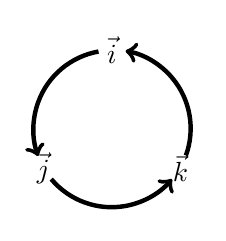
\begin{tikzpicture}
  \draw[ultra thick,->] (.94,-.34) arc (-20:80:1cm);
  \draw[ultra thick,->] (-.17,.98) arc (100:200:1cm);
  \draw[ultra thick,->] (-.77,-.64) arc (220:320:1cm);
  \node at (0,1) {$\vec{i}$};
  \node at (-.87,-.5) {$\vec{j}$};
  \node at (.87,-.5) {$\vec{k}$};
\end{tikzpicture}
\end{image}

Since we see that the cross product of two basic unit vectors produces
a vector orthogonal to \textit{both} unit vectors, we are lead to our
next theorem (which could be verified through brute force
computations).

\begin{theorem}
  The vector $\vec{v}\times\vec{w}$ is orthogonal to both $\vec{v}$
  and $\vec{w}$.
\end{theorem}

When seeking a vector perpendicular to both $\vec v$ and $\vec w$, we
essentially have two directions to choose from, one in the direction
of $\vec{v}\times\vec{w}$ and one in the direction of
$\vec{w}\times\vec{v}$.  The direction of the cross product is given
by the \textit{right hand rule}.  Given $\vec{a}$ and $\vec{b}$ in
$\R^3$ with the same initial point, point the index finger of your
right hand in the direction of $\vec{a}$ and let your middle finger
point in the direction of $\vec{b}$ (much as we did when establishing
the right hand rule for the 3-dimensional coordinate system). Your
thumb will naturally extend in the direction of
$\vec{a}\times\vec{b}$.  If you switch, and point the index finder in
the direction of $\vec{b}$ and the middle finger in the direction of
$\vec{a}$, your thumb will now point in the opposite direction,
allowing you to ``visualize'' the anticommutative property of the
cross product.
\begin{image}
  %% Based on: https://commons.wikimedia.org/wiki/File:Right_hand_rule_cross_product.svg
  %% Which was based on: https://commons.wikimedia.org/wiki/File:Right_hand_cross_product.png
  %% Which was based on: https://commons.wikimedia.org/wiki/File:LeftHandOutline.png
  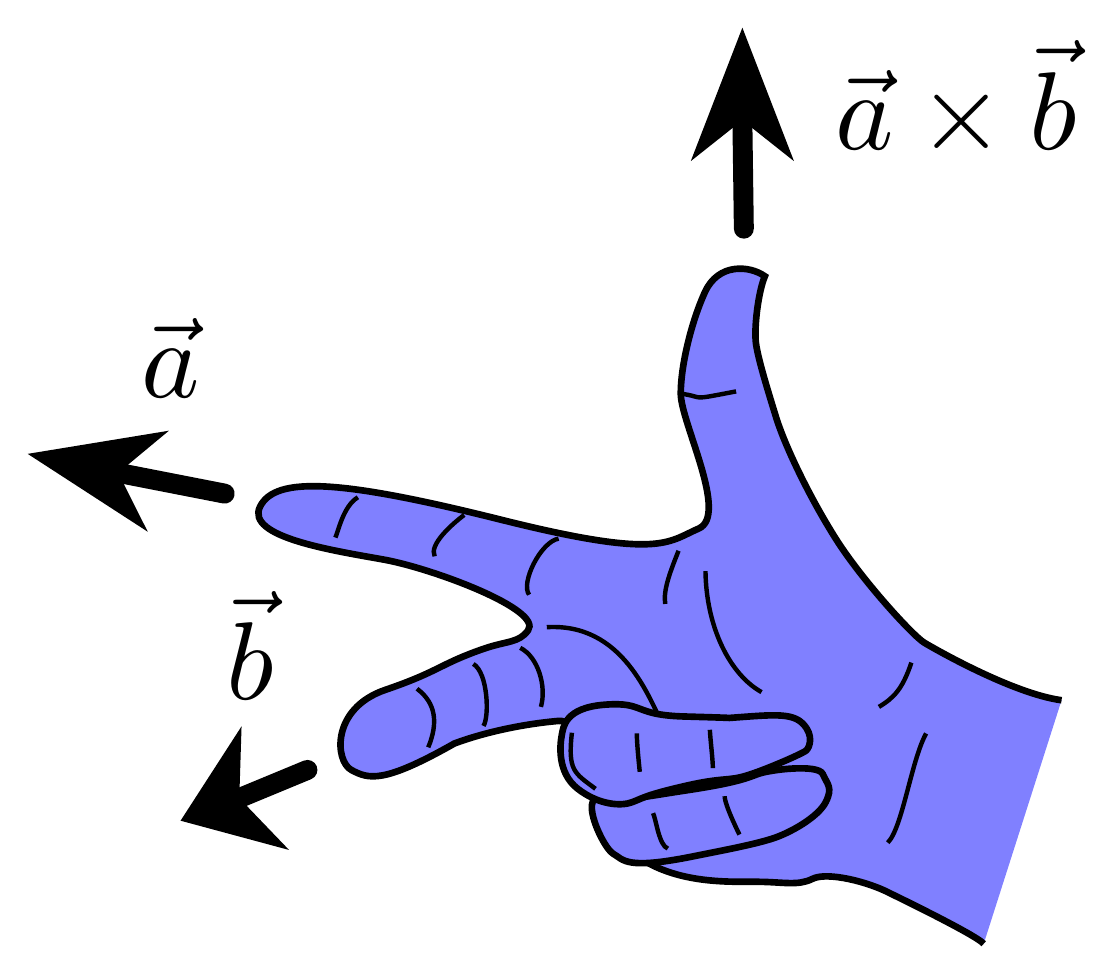
\begin{tikzpicture}[y=0.80pt, x=0.80pt, yscale=-1.000000, xscale=1.000000, inner sep=0pt, outer sep=0pt]
    \path[draw=black,fill=blue!50!white,line width=2.400pt] (466.9820,303.7880) ..
    controls (444.9820,300.7880) and (409.9820,280.7880) .. (404.9820,277.7880) ..
  controls (399.9820,274.7880) and (376.9820,249.7880) .. (364.9820,230.7880) ..
  controls (352.9820,211.7880) and (341.9820,188.7880) .. (337.9820,175.7880) ..
  controls (333.9820,162.7880) and (329.9820,149.7880) .. (328.9820,142.7880) ..
  controls (327.9820,135.7880) and (329.9820,119.2880) .. (332.9820,112.2880) ..
  controls (325.9820,107.2880) and (311.9820,106.2880) .. (305.9820,119.2880) ..
  controls (299.9820,132.2880) and (294.9820,152.2880) .. (294.9820,165.2880) ..
  controls (294.9820,178.2880) and (316.9820,220.2880) .. (302.9820,226.2880) ..
  controls (288.9820,232.2880) and (285.9820,240.2880) .. (213.9820,222.2880) ..
  controls (141.9820,204.2880) and (111.9820,202.2880) .. (104.9820,216.2880) ..
  controls (97.9820,230.2880) and (138.9820,236.2880) .. (160.9820,240.2880) ..
  controls (182.9820,244.2880) and (233.0030,262.9220) .. (225.9820,272.2880) ..
  controls (221.6320,278.0900) and (216.6070,276.7760) .. (205.2730,280.7760) ..
  controls (185.6620,287.6980) and (185.9650,290.7420) .. (161.4820,299.1210) ..
  controls (137.0490,307.4830) and (138.6390,331.3470) .. (146.3150,335.3510) ..
  controls (153.9910,339.3550) and (160.3310,341.6930) .. (192.7010,323.3380) ..
  controls (207.0510,317.9980) and (224.4830,314.4530) .. (239.8160,313.1200) ..
  controls (255.1490,311.7870) and (264.4840,369.1200) .. (281.1500,377.7870) ..
  controls (297.8160,386.4540) and (317.1490,385.7870) .. (329.1490,385.7870) ..
  controls (341.1490,385.7870) and (347.8150,387.7880) .. (354.4820,384.4540) ..
  controls (361.1490,381.1200) and (379.8160,385.7860) .. (389.8160,391.1200) ..
  controls (389.8160,391.1200) and (428.4830,409.7870) .. (431.8160,413.7870);
\path[draw=black,line width=1.600pt] (234.4830,270.7870) .. controls
  (268.4820,268.7880) and (280.4820,301.4540) .. (288.4820,318.7880);
\path[draw=black,line width=1.600pt] (306.1490,245.4530) .. controls
  (306.4830,270.7870) and (317.1500,292.1210) .. (331.4820,300.1190);
\path[draw=black,line width=1.600pt] (239.8160,230.7870) .. controls
  (231.8160,232.1200) and (222.4830,250.7870) .. (226.4830,256.1200);
\path[draw=black,line width=1.600pt] (197.1490,220.1200) .. controls
  (191.8160,224.1200) and (181.1490,233.4530) .. (183.8160,238.7870);
\path[draw=black,line width=1.600pt] (149.1490,212.1200) .. controls
  (142.4820,216.1200) and (140.3150,227.6210) .. (138.9820,230.2870);
\path[draw=black,line width=1.600pt] (222.4830,280.1210) .. controls
  (230.4830,284.1210) and (234.4830,297.4530) .. (231.8160,306.7870);
\path[draw=black,line width=1.600pt] (201.2960,287.3930) .. controls
  (207.9630,291.3930) and (208.5440,311.3860) .. (205.8770,315.3860);
\path[draw=black,line width=1.600pt] (175.8480,298.5900) .. controls
  (184.4960,305.0750) and (185.4390,314.1240) .. (180.9370,325.0560);
\path[draw=black,line width=1.600pt] (293.9820,236.2880) .. controls
  (289.9820,246.2880) and (286.9820,254.2880) .. (287.9820,260.2880);
\path[draw=black,line width=1.600pt] (294.9820,165.2880) .. controls
  (306.9290,166.9950) and (297.6590,168.5400) .. (319.9820,164.2880);
\path[draw=black,line width=1.600pt] (399.1490,286.7880) .. controls
  (395.1490,298.7880) and (391.1490,302.7870) .. (384.4820,306.7870);
\path[draw=black,fill=blue!50!white,line width=2.400pt] (299.8160,374.4550) ..
  controls (315.7210,371.2740) and (327.1500,369.1220) .. (335.8160,366.4550) ..
  controls (344.4820,363.7880) and (357.1480,356.4540) .. (360.4820,349.7880) ..
  controls (363.8160,343.1220) and (361.1490,341.7890) .. (359.1490,337.1220) ..
  controls (357.1490,332.4550) and (335.1500,335.1220) .. (329.8160,337.1220) ..
  controls (324.4820,339.1220) and (319.8160,341.1220) .. (297.8160,344.4550) ..
  controls (275.8160,347.7880) and (269.8160,349.4550) .. (258.4820,348.1210) ..
  controls (249.1900,347.0270) and (259.8170,370.4540) .. (264.4830,373.1210) ..
  controls (269.1490,375.7880) and (269.8160,380.4550) .. (299.8160,374.4550) --
  cycle;
\path[draw=black,fill=blue!50!white,line width=2.400pt] (316.7840,311.7880) ..
  controls (335.6810,310.4550) and (345.1320,309.1220) .. (350.2190,314.4550) ..
  controls (355.3060,319.7880) and (353.1250,325.1220) .. (351.6720,326.4550) ..
  controls (350.2190,327.7880) and (333.5010,335.1210) .. (324.7790,337.7880) ..
  controls (316.0560,340.4550) and (314.6030,338.4550) .. (297.1600,342.4550) ..
  controls (279.7160,346.4550) and (278.2630,347.7880) .. (273.1740,349.7880) ..
  controls (268.0860,351.7880) and (257.9110,351.1210) .. (248.4630,343.7880) ..
  controls (239.0140,336.4550) and (240.4670,323.7880) .. (241.1940,319.7880) ..
  controls (241.9210,315.7880) and (242.6490,307.1210) .. (260.8190,305.7880) ..
  controls (278.9890,304.4550) and (273.1730,310.4540) .. (296.4330,311.1210) ..
  controls (319.6910,311.7880) and (316.7840,311.7880) .. (316.7840,311.7880) --
  cycle;
\path[draw=black,line width=1.600pt] (245.8150,318.4550) .. controls
  (243.8920,335.7600) and (246.9240,336.6210) .. (256.4820,343.7880);
\path[draw=black,line width=1.600pt] (275.1490,318.7870) .. controls
  (275.1490,324.1200) and (276.4820,336.1200) .. (276.4820,336.1200);
\path[draw=black,line width=1.600pt] (308.1490,317.1200) .. controls
  (308.1490,319.7870) and (309.4830,330.4530) .. (309.4830,334.4530);
\path[draw=black,line width=1.600pt] (314.8150,347.1220) .. controls
  (314.8150,351.1220) and (321.4820,364.4550) .. (321.4820,364.4550);
\path[draw=black,line width=1.600pt] (282.4820,354.7880) .. controls
  (283.8150,357.4550) and (285.1490,369.4540) .. (289.1490,370.7880);
\path[draw=black,line width=1.600pt] (405.8150,318.7880) .. controls
  (399.1490,330.7880) and (395.1490,361.4560) .. (388.4820,368.1220);
\path[draw=black,fill=black,line cap=round,line width=7.200pt]
  (323.4820,90.7880) -- (322.8140,41.7880);
\path[fill=black] (322.8140,41.7880) -- (299.5010,60.3000) -- (322.8140,0.0000)
  -- (346.1270,60.3000) -- cycle;
\path[draw=black,fill=black,line cap=round,line width=7.200pt]
  (88.9960,210.4600) -- (40.9000,201.0670);
\path[fill=black] (40.9000,201.0670) -- (54.2400,227.6800) -- (0.0000,192.5000)
  -- (63.7990,182.0440) -- cycle;
\path[draw=black,fill=black,line cap=round,line width=7.200pt]
  (126.3770,335.2550) -- (95.5850,348.0050);
\path[fill=black] (95.5850,348.0050) -- (118.0640,371.4130) --
  (69.0630,358.1970) -- (96.6050,315.5680) -- cycle;
\path[fill=black,line join=miter,line cap=butt,line width=0.800pt]
  (51.2201,166.8365) node[above right] (text4204) {\scalebox{4}{$\vec{a}$}};
\path[fill=black,line join=miter,line cap=butt,line width=0.800pt]
  (89.7117,303.4817) node[above right] (text4208) {\scalebox{4}{$\vec{b}$}};
\path[fill=black,line join=miter,line cap=butt,line width=0.800pt]
  (364.9268,59.0600) node[above right] (text4212) {\scalebox{4}{$\vec{a}\times\vec{b}$}};
\end{tikzpicture}
\end{image}


\begin{question}
  Consider the vectors below:
  
  Is BLANK pointing toward you or away from you?
\end{question}




This formula is pretty horrible, and you may be wondering why anyone
would ever care about such a thing.  The answer is that is has a very
nice relationship to the determinate, and hence to volumes, areas, and
orientations:

\begin{theorem}[Triple product theorem]
  If $\vec{a},\vec{b},$ and $\vec{c}$ are vectors in $\R^3$, then 
  
  \[
  (\vec{a} \times \vec{b}) \cdot \vec{c} = \det(\vec{a},\vec{b},\vec{c}) 
  \]
\end{theorem}

\begin{proof}
  
  The proof is just a computation:
  
  \begin{align*}
    (\vec{a} \times \vec{b}) \cdot \vec{c} &= \vector{a_2b_3-a_3b_2, -(a_1b_3-a_3b_1), a_1b_2-a_2b_1} \cdot \vector{c_1,c_2,c_3}\\
    &=c_1a_2b_3-c_1a_3b_2+c_2a_3b_1-c_2a_1b_3+c_3a_1b_2-c_3a_2b_1\\
    &=\det(\vec{a},\vec{b},\vec{c}) 
  \end{align*}
\end{proof}

This theorem will allow us to gain massive insight into the geometric nature of the cross product:

\begin{theorem}
  $\vec{a} \times \vec{b}$ is perpendicular to both $\vec{a}$ and $\vec{b}$.
\end{theorem}

\begin{proof}
  We need to show that $(\vec{a} \times \vec{b}) \cdot \vec{a} = 0 $ and $\vec{a} \times \vec{b} \cdot \vec{b} = 0$.  Let's just do the first one:
  
  \[
  (\vec{a} \times \vec{b}) \cdot \vec{a} = \det(\vec{a},\vec{b},\vec{a})
  \]
  
  But this must be zero by the alternating property.
	
  The other case follows similarly.
\end{proof}


\section{The geometry of the cross product}

Just as we related the angle between two vectors and their dot
product, there is a similar relationship relating the cross product of
two vectors to the angle between them.

\begin{theorem}[Geometric Interpretation of the Cross Product]\index{cross product}
  For any two vectors $\vec{v}$ and $\vec{w}$,
  \[
  |\vec{v} \times \vec{w}| = |\vec{v}||\vec{w}|\sin(\theta)
  \]
  where $0\le \theta\le\pi$ is the angle between $\vec{v}$ and
  $\vec{w}$.
\end{theorem}

\begin{theorem}
  If $\vec{v}$ and $\vec{w}$ are two nonzero vectors, and $\theta$ is
  the angle between them,
  \[
  \vec{v}\times \vec{w} = 0 \text{ if and only if $\theta=
  0$ or $\theta=\pi$}.
  \]
\end{theorem}

This theorem tells us that the cross product of nonzero parallel
vectors is $\vec{0}$.



\begin{theorem}
  The length of $\vec{a} \times \vec{b}$ is the area of the
  parallelogram spanned by $\vec{a}$ and $\vec{b}$.  Also the trio
  $(\vec{a},\vec{b},\vec{a} \times \vec{b})$ is positively oriented.
\end{theorem}

\begin{proof}
  \begin{align*}
    |\vec{a} \times \vec{b}|^2  &=(\vec{a} \times \vec{b}) \cdot (\vec{a} \times \vec{b})\\
    &=\det(\vec{a},\vec{b},\vec{a} \times \vec{b})
  \end{align*}
  
  Note that this already shows that the trio is positively oriented,
  since the determinant $\det(\vec{a},\vec{b},\vec{a} \times \vec{b})$
  is equal to the square of a length, which must be positive.
  
  Also note that $\det(\vec{a},\vec{b},\vec{a} \times \vec{b})$
  represents the volume of the parallelepiped spanned by $\vec{a}$,
  $\vec{b}$, and $\vec{a} \times \vec{b}$.  Since we already know that
  $vec{a} \times \vec{b}$ is perpendicular to the plane spanned by
  $\vec{a}$ and $\vec{b}$, then just by geometry (base times height)
  we know that this volume is equal to $A |vec{a} \times \vec{b}|$,
  where $A$ is the area of the parallelogram spanned by $\vec{a}$ and
  $\vec{b}$.  Hence
  \[
  |\vec{a} \times \vec{b}|^2 = A |\vec{a} \times \vec{b}|
  \]
  From which the claim follows.
\end{proof}

\begin{question}
  What is the area of the parallelogram spanned by $\vector{1,2,4}$ and $\vector{2,3,1}$?
  \[
  \textrm{Area} = \answer{\sqrt{150}}
  \]
  
  \begin{hint}
    \[
    \vector{1,2,4} \times \vector{2,3,1} = \vector{-10,7,-1}
    \]
  \end{hint}
  
  
  \begin{hint}
    \begin{align*}
      \left| \vector{-10,7,-1} \right| &= \sqrt{ \vector{-10,7,-1} \cdot  \vector{-10,7,-1}}\\
      &=\sqrt{100+49+1}\\
      &=\sqrt{150}
    \end{align*}
    
    Since the area of the parallelogram is the length of the cross product, we are done.
  \end{hint}
\end{question}

AREA OF TRIANGLE (SOMEHOW WE NEED TO connect $|\vec{u}\times\vec{v}$  to det of 2x2 matrix



Putting all of these ideas together we have:

\begin{theorem}
  $\vec{a} \times \vec{b}$ is the vector perpendicular to the plane
  spanned by $\vec{a}$ and $\vec{b}$ which points in the ``positive
  direction'', as given by the right hand rule, and whose length is
  the area of the parallelogram spanned by $\vec{a}$ and $\vec{b}$.
\end{theorem}

\begin{observation}
  Since the height of this parallelogram is $|\vec{b}| \sin\theta$ and
  its length is $|\vec{a}|$ where $\theta$ is the angle between
  $\vec{a}$ and $\vec{b}$, we could also say that $|\vec{a} \times
  \vec{b}| = |\vec{a}||vec{b}| \sin\theta$
\end{observation}

\begin{question}
  Using the geometric ideas above, compute the following cross
  products.  It may be helpful to use your left hand to form a
  coordinate system (where your index finger is the positive $z$ axis,
  your thumb is the positive $x$ axis, and your middle finger is the
  positive $y$ axis), and use your right hand to determine
  orientation.
  
  \begin{align*}
    \vector{1,0,0} \times \vector{0,1,0} = \vector{\answer{0},\answer{0},\answer{1}}\\
    \vector{0,1,0} \times \vector{1,0,0} = \vector{\answer{0},\answer{0},\answer{-1}}\\
    \vector{0,0,1} \times \vector{0,1,0} = \vector{\answer{-1},\answer{0},\answer{0}}\\
    \vector{0,1,0} \times \vector{0,1,0} = \vector{\answer{0},\answer{0},\answer{0}}\\
  \end{align*}
\end{question}

Below, we summarize some rules for working with cross products:

\begin{theorem}
  
  Let $\vec{v},\vec{w},\vec{u} \in \R^3$.  Then
  
  \begin{itemize}
  \item $\vec{v} \times \vec{w}  = -\vec{w} \times \vec{v}$ (Anti-commutivity property )
  \item $(\vec{v}+\vec{w}) \times \vec{u} = \vec{v} \times \vec{u}+\vec{w} \times \vec{u}$ (Right distributive property)
  \item $\vec{u} \times (\vec{v} +\vec{w}) = \vec{u} \times \vec{v}+\vec{u}\times\vec{w}$ (Left distributive property)
  \item $a\vec{v} \times b\vec{w} = ab \vec{v} \times \vec{w}$ (Respects scalar multiplication)
  \item $\vec{v} \times \vec{v} = 0$
  \item $\vec{i} \times \vec{j} = \vec{k}$
  \item $\vec{i} \times \vec{k} = \vec{-j}$
  \item $\vec{j} \times \vec{k} = \vec{i}$
  \end{itemize}
  
  Moreover, these properties determine the cross product uniquely.
\end{theorem}

\begin{question}
  Using only these rules, compute $(3\vec{i}+k) \times (2\vec{j}+\vec{i})$
  \[
  (3\vec{i}+\vec{k}) \times (2\vec{j}+\vec{i}) = \answer{-2}\vec{i}+\answer{1}\vec{j}+\answer{6}\vec{k}
  \]
  \begin{hint}
    \begin{align*}
      (3\vec{i}+\vec{k}) \times (2\vec{j}+\vec{i}) &= (3\vec{i}+\vec{k}) \times 2\vec{j}+(3\vec{i}+\vec{k}) \times\vec{i}\\
      &=3\vec{i} \times 2\vec{j}+\vec{k}\times 2\vec{j}+3\vec{i} \times \vec{i} +\vec{k} \times \vec{i}\\
      &=6 \vec{i} \times \vec{j}+2 \vec{k} \times \vec{j}+3\vec{i} \times \vec{i} +\vec{k} \times \vec{i}\\
      &=6 \vec{i} \times \vec{j}+-2 \vec{j} \times \vec{k}+3\vec{i} \times \vec{i} -\vec{i} \times \vec{k}\\
      &=6 \vec{k}+-2 \vec{i}+3\vec{0} -(-\vec{j})\\
      &=-2\vec{i}+1\vec{j}+6\vec{k}
    \end{align*}
  \end{hint}
\end{question}



\section{Applications}

In addition to the geometric applications we have already seen
(calculating the area of parallelograms), we can also use the cross
product in some physical applications.

\subsection{Torque}

Imagine turning a wrench.  The wrench originates at a point $O$ and
terminates at a point $P$.  Let $\vec{r} = \overrightarrow{OP}$.  You
apply a force $\vec{F}$ to the end of the wrench.  If $\vec{F}$ points
in the same direction as $\vec{r}$, the bolt will not twist at all,
since you will just be pulling on the handle.  If $\vec{F}$ is
perpendicular to the handle, then we expect quite a bit of twisting to
occur.

\begin{definition}
  The torque $\vec{\tau}$ obtained by applying a force $\vec{F}$ to a lever arm with position vector $\vec{r}$ is given by
  \[
  \vec{\tau} = \vec{r} \times \vec{F} 
  \]
\end{definition}

\begin{question}
  A pipe of length $3 \unit{m}$ has a force of magnitude $2 \unit{N}$
  applied to it as shown below:
  
  \begin{image}
    \begin{tikzpicture}
      \begin{axis}[
          xmin=-1,xmax=5,ymin=-1,ymax=3,
          clip=false,
          axis lines=center,
          ticks=none,
          unit vector ratio*=1 1 1,
          xlabel=$x$, ylabel=$y$,
          %ytick={-2,-1,...,7},
	  %xtick={-2,-1,...,10},
	  % grid = major,
          every axis y label/.style={at=(current axis.above origin),anchor=south},
          every axis x label/.style={at=(current axis.right of origin),anchor=west},
        ]
        \addplot[very thick,penColor,->] plot coordinates {(0,0) (1,2)};
        \addplot[very thick,penColor2,->] plot coordinates {(1,2) (0.5,3)};
        \addplot[very thick,penColor, dashed] plot coordinates {(1,2) (2,4)};
        \node at (axis cs:1, 2.6) [textColor] {$\frac{\pi}{3}$};
        \node at (axis cs:0.6, 0.7) [penColor] {$\vec{r}$};
        \node at (axis cs:0.6, 2.4) [penColor2] {$\vec{F}$};
      \end{axis}
    \end{tikzpicture}
  \end{image}
  Assuming the $z$-axis is coming towards you (out of the page), is
  the torque produced in the positive or negative $z$ direction?

  \begin{multipleChoice}
    \choice[correct]{positive}
    \choice{negative}
  \end{multipleChoice}
  \[
  |\vec{tau}| = \answer{3\sqrt{3}}
  \]
  \begin{hint}
    Using the right hand rule, we see that the vector points in the
    positive $z$ direction.
  \end{hint}
  \begin{hint}
    The angle between the two vectors is $\frac{\pi}{3}$, so the area
    of the area of the parallelogram spanned by these vectors is
    $2(3)\sin(\frac{\pi}{3}) = 3\sqrt{3}$
  \end{hint}
  
\end{question}

\subsection{Magnetism} 

When a charged particle moves through a magnetic field, it experiences a force.  If the charge is $q$, the velocity of the particle is $\vec{v}$, and the magnetic field is $\vec{B}$, then the force is given by

\[
\vec{F} = q\vec{v} \times \vec{B}
\]

\begin{question}
	A particle with negative charge $-2$ enters a constant magnetic field given by $\vec{B} = \vec{i}+2\vec{j}$.  The velocity vector of the particle is  $\vec{v} = \vec{k}+\vec{i}$.  What is the force acting on the particle?
	
	\[
	\vec{F} = \answer{4}\vec{i}+\answer{-2}\vec{j}+\answer{-2}\vec{k}
	\]
	
	\begin{hint}
		\begin{align*}
			\vec{F} &= q\vec{v} \times \vec{B}\\
				&= -2 ( \vec{k}+\vec{i}) \times (\vec{i}+2\vec{j})\\
				&=-2( \vec{k} \times \vec{i}+2\vec{k} \times \vec{j}+\vec{i} \times \vec{i}+\vec{i} \times \vec{j})\\
				&=-2(\vec{j}-2\vec{i}+\vec{0}+\vec{k})\\
				&=4\vec{i}-2\vec{j}-2\vec{k}
		\end{align*}
	\end{hint}
\end{question}





\url{http://www.jstor.org/discover/10.2307/2323537?uid=3739256&uid=2&uid=4&sid=21103780384137}

















\begin{question}
  If $\det(\vec{a},\vec{b},\vec{c}) = 12$, what is
  $\det(\vec{b},\vec{a},\vec{c})$?
  \[
  \det(\vec{b},\vec{a},\vec{c}) = \answer{-12}
  \]
  \begin{hint}
    \[
    \begin{vmatrix} 
      b_1 & a_1 & c_1\\
      b_2 & a_2 & c_2\\
      b_3 & a_3 & c_3\\
    \end{vmatrix}
    =b_1a_2c_3+a_2c_3b_3+c_1b_2a_3-b_3a_2c_1-a_3c_3b_1-c_3b_2a_1
    \]
    
    But this (make sure you check!) equal to
    $-\det(\vec{a},\vec{b},\vec{c})$.  Thus the answer is $-12$.
  \end{hint}
\end{question}

\begin{question}
  \[
  \det(\vec{a},\vec{a},\vec{b}) = \answer{0}
  \]
  \begin{hint}
    If you write out the definition, you will see that all the terms cancel, and you get $0$
  \end{hint}
\end{question}
	
\begin{question}
  Assume $\det(\vec{a},\vec{b},\vec{c}) = 3$.  Then 
  \[
  \det(5\vec{a},\vec{b},2\vec{c}) = \answer{30}
  \]
  \begin{hint}
    Since each term has an entry from $\vec{a},\vec{b}$ and $\vec{c}$,
    and each entry of each vector is getting multiplied by the same
    constant, we get an extra factor of $10$ in each term.  Thus the
    answer is $30$.
  \end{hint}
\end{question}

\begin{question}
  Assume $\det(\vec{a},\vec{b},\vec{c}) = 3$ and
  $\det(\vec{a},\vec{b},\vec{d}) = 4$.
  \[
  \det(\vec{a},\vec{b},\vec{c}+\vec{d}) = \answer{7}
  \]
  
  \begin{hint}
    Writing out the definition, and distributing, you will see that
    this is equal to the sum of the two original determinants.  So the
    answer is $7$.
  \end{hint}
\end{question}

The last few exercises strongly suggest the following theorem (which you have essentially already proven by doing the exercises above):
	
\begin{theorem}
  The determinant enjoys the following properties, and is in fact the
  \textbf{only} function enjoying such properties:
  
  \begin{itemize}
  \item Alternating: Switching any pair of entries in the determinant
    switches the sign.  For example $\det(\vec{a},\vec{b},\vec{c}) =
    -\det(\vec{c},\vec{b},\vec{a})$.
  \item Factor out scalars: Multiplying any entry by a constant scales
    the determinant by that constant.  For example
    $\det(k\vec{a},\vec{b},\vec{c}) = k\det(\vec{a},\vec{b},\vec{c})$
  \item Respect addition: For example
    $\det(\vec{a},\vec{b}+\vec{d},\vec{c}) =
    \det(\vec{a},\vec{b},\vec{c}) +\det(\vec{a},\vec{d},\vec{c}) $
  \item $\det(\vec{i},\vec{j},\vec{k}) = 1 $
  \end{itemize}
\end{theorem}

\begin{observation}
  By the alternating property, if the same vector appears more than
  once as an argument in a determinant, then the determinant must be
  zero.  For example consider $\det(\vec{a},\vec{a},\vec{b})$. By the
  alternating property we must have
  \[
  \det(\vec{a},\vec{a},\vec{b}) = -\det(\vec{a},\vec{a},\vec{b})
  \]
  but this implies 
  
  \[
  \det(\vec{a},\vec{a},\vec{b})=0
  \]
\end{observation}
	
We will not prove that the determinant is the only function with these
properties, but that is an important point.  If you ever wondered
where this crazy formula came from, this explains it.  If you want
these $4$ nice looking properties, there is only one function which
does it and it is this one.  You should be able to prove that
yourself, using just the properties.  Just start with a general
$\det(\vec{a},\vec{b},\vec{c}) $, and use the properties to reduce it
to sums of determinants involving only $\vec{i},\vec{j}$ and
$\vec{k}$.  The formula for the determinant will pop out.
	
It turns out that the determinant has the following geometric
interpretation:
\begin{theorem}
  If $\vec{a},\vec{b},\vec{c} \in \R^3$, then they span a
  parallelepiped. The volume of this parallelepiped is
  $\left|\det(\vec{a},\vec{b},\vec{c})\right|$. If this parallelepiped
  is not degenerate (has nonzero volume), then the sign of
  $\det(\vec{a},\vec{b},\vec{c})$ tells you whether the trio of
  vectors is \dfn{positively oriented} or \dfn{negatively oriented}
  (this is the definition of positively and negatively oriented).
\end{theorem} 
	
\begin{question}
  Let $\vec{a} = \vector{1,1,1}$, $\vec{b} = \vector{1,0,1}$ and
  $\vec{c} = \vector{1,0,0}$.  Is $(\vec{a},\vec{b},\vec{c})$
  positively or negatively oriented?
  \begin{multipleChoice}
    \choice[correct]{positively}
    \choice{negatively}
  \end{multipleChoice}
		
  What is the volume of the parallelepiped spanned by these three vectors?
  
  \[
  \textrm{Volume} = \answer{1}
  \]
  
  \begin{hint}
    \begin{align*}
      \begin{vmatrix}
	1 & 1 & 1\\
	1 & 0 & 0\\
	1 & 1 & 0
      \end{vmatrix} &=
      1(0)(0)+1(0)(1)+1(1)(1)-1(0)(1)-1(1)(1)-0(1)(1)\\
      &=1
    \end{align*}
    
    Thus this trio is positively oriented, and its volume is $1$.
  \end{hint}
\end{question}

\begin{question}
  Do the vectors $\vector{1,2,2}$, $\vector{3,4,1}$ and $\vector{5,8,5}$ all lie in the same plane?
  
  \begin{multipleChoice}
    \choice{No}
    \choice[correct]{Yes}
  \end{multipleChoice}
  
  \begin{hint}
    They will lie in the same plane if and only if the parallelepiped they span
    is degenerate, aka its volume is $0$.
  \end{hint}
  
  \begin{hint}
    So we just need to see whether the determinant of these three
    vectors is zero or not.
  \end{hint}
  
  \begin{hint}
    \begin{align*}
      \begin{vmatrix}
	1&3&5\\
	2&4&8\\
	2&1&5
      \end{vmatrix} &= 1(4)(5)+3(8)(2)+5(2)(1)-2(4)(5)-1(8)(1)-5(2)(3)\\
      &=20+48+10-40-8-30\\
      &=78-78\\
      &=0
    \end{align*}
    
    Thus the vectors must all lie in the same plane.  In fact, we can
    see that $2\vector{1,2,2}+\vector{3,4,1}=\vector{5,8,5}$, which
    confirms this fact.
  \end{hint}
  
\end{question}
We will not explicitly prove this theorem here.  However, you
should be able to convince yourself that the oriented volume
function $\textrm{Vol}(\vec{a},\vec{b},\vec{c})$ satisfies all
$4$ conditions of the determinant above.  Since there is only
one function satisfying these properties, the volume function
must be given by the determinant.
Here is a nice geometric interpretation of orientation.

\begin{theorem}
  Consider the trio of vectors $(\vec{a},\vec{b},\vec{c})$.  Assume
  that they form a nondegenerate parallelepiped.  Then the vectors
  $\vec{a}$ and $\vec{b}$ define a plane.  There are two sides to this
  plane.  If you take your right hand, and curl your fingers from
  $\vec{a}$ to $\vec{b}$, your thumb will be pointing to one side of
  the plane.  If $\vec{c}$ is on this side, then the trio is
  positively oriented.  Otherwise it is negatively oriented.
  \begin{center}
    BADBAD
    %\includegraphics[width=3 in]{RHR.jpg}
    All vectors on the same side of the plane that the thumb is pointing are positively oriented with respect to $(A,B)$
  \end{center}
\end{theorem}








\end{document}
